\documentclass[border=6pt]{standalone}
\usepackage[utf8]{inputenc}\usepackage[T1]{fontenc}\usepackage{lmodern}\usepackage[english]{babel}
\usepackage{amsmath,amssymb}\usepackage{tikz}\usetikzlibrary{arrows.meta,positioning,calc}
\begin{document}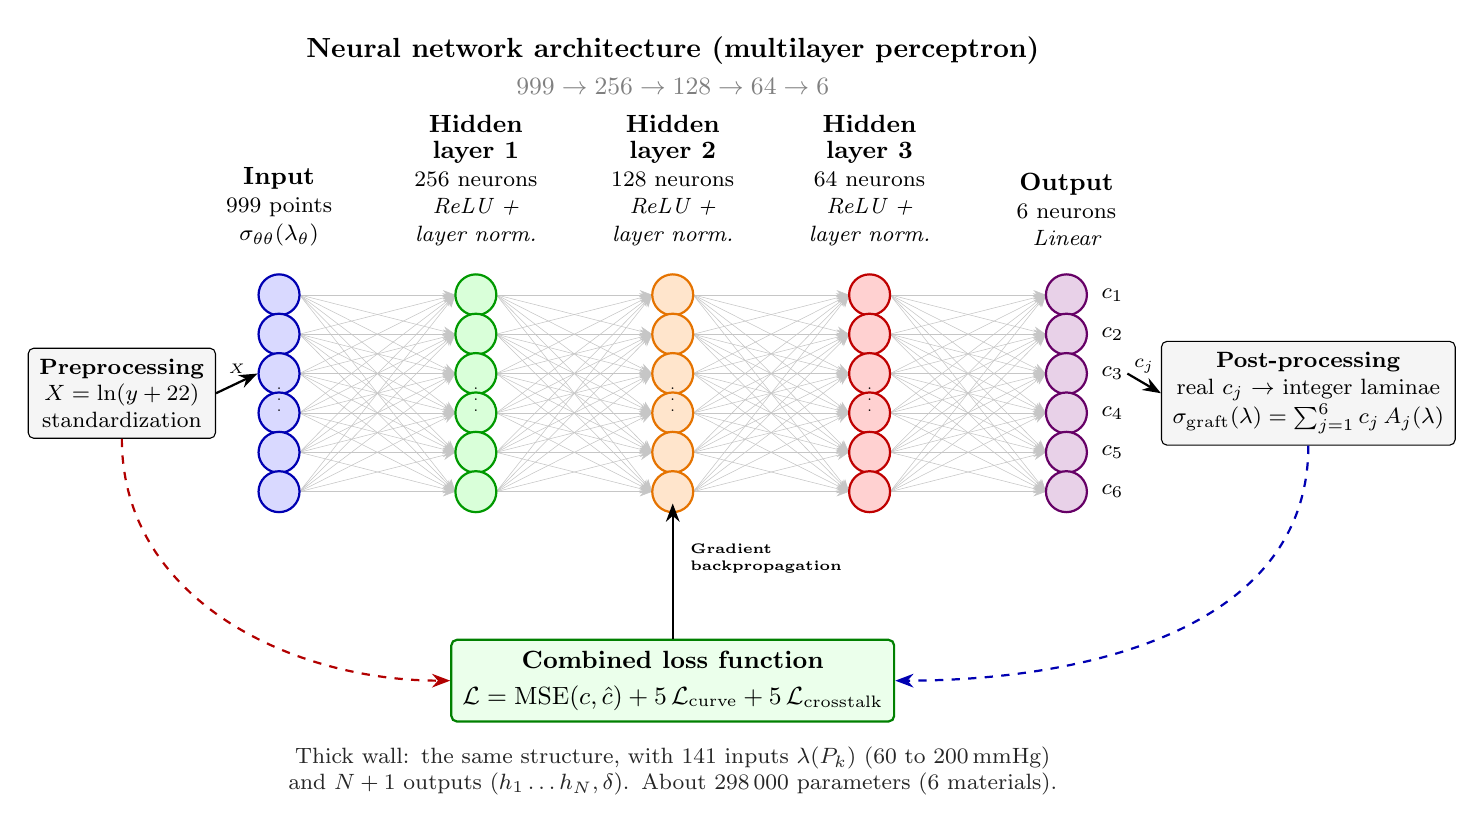
\begin{tikzpicture}[font=\small, n/.style={circle,draw,thick,minimum size=5.2mm,inner sep=0pt},
 box/.style={draw,rounded corners=2pt,fill=gray!8,align=center,inner sep=4pt,font=\footnotesize}]

\node[font=\bfseries\normalsize] at (5.0,5.6) {Neural network architecture (multilayer perceptron)};
\node[gray] at (5.0,5.15) {$999\to256\to128\to64\to6$};
\draw[-{Stealth[length=1.6mm]},gray!45,very thin] (0.26,2.50)--(2.24,2.50);
\draw[-{Stealth[length=1.6mm]},gray!45,very thin] (0.26,2.50)--(2.24,2.00);
\draw[-{Stealth[length=1.6mm]},gray!45,very thin] (0.26,2.50)--(2.24,1.50);
\draw[-{Stealth[length=1.6mm]},gray!45,very thin] (0.26,2.50)--(2.24,1.00);
\draw[-{Stealth[length=1.6mm]},gray!45,very thin] (0.26,2.50)--(2.24,0.50);
\draw[-{Stealth[length=1.6mm]},gray!45,very thin] (0.26,2.50)--(2.24,0.00);
\draw[-{Stealth[length=1.6mm]},gray!45,very thin] (0.26,2.00)--(2.24,2.50);
\draw[-{Stealth[length=1.6mm]},gray!45,very thin] (0.26,2.00)--(2.24,2.00);
\draw[-{Stealth[length=1.6mm]},gray!45,very thin] (0.26,2.00)--(2.24,1.50);
\draw[-{Stealth[length=1.6mm]},gray!45,very thin] (0.26,2.00)--(2.24,1.00);
\draw[-{Stealth[length=1.6mm]},gray!45,very thin] (0.26,2.00)--(2.24,0.50);
\draw[-{Stealth[length=1.6mm]},gray!45,very thin] (0.26,2.00)--(2.24,0.00);
\draw[-{Stealth[length=1.6mm]},gray!45,very thin] (0.26,1.50)--(2.24,2.50);
\draw[-{Stealth[length=1.6mm]},gray!45,very thin] (0.26,1.50)--(2.24,2.00);
\draw[-{Stealth[length=1.6mm]},gray!45,very thin] (0.26,1.50)--(2.24,1.50);
\draw[-{Stealth[length=1.6mm]},gray!45,very thin] (0.26,1.50)--(2.24,1.00);
\draw[-{Stealth[length=1.6mm]},gray!45,very thin] (0.26,1.50)--(2.24,0.50);
\draw[-{Stealth[length=1.6mm]},gray!45,very thin] (0.26,1.50)--(2.24,0.00);
\draw[-{Stealth[length=1.6mm]},gray!45,very thin] (0.26,1.00)--(2.24,2.50);
\draw[-{Stealth[length=1.6mm]},gray!45,very thin] (0.26,1.00)--(2.24,2.00);
\draw[-{Stealth[length=1.6mm]},gray!45,very thin] (0.26,1.00)--(2.24,1.50);
\draw[-{Stealth[length=1.6mm]},gray!45,very thin] (0.26,1.00)--(2.24,1.00);
\draw[-{Stealth[length=1.6mm]},gray!45,very thin] (0.26,1.00)--(2.24,0.50);
\draw[-{Stealth[length=1.6mm]},gray!45,very thin] (0.26,1.00)--(2.24,0.00);
\draw[-{Stealth[length=1.6mm]},gray!45,very thin] (0.26,0.50)--(2.24,2.50);
\draw[-{Stealth[length=1.6mm]},gray!45,very thin] (0.26,0.50)--(2.24,2.00);
\draw[-{Stealth[length=1.6mm]},gray!45,very thin] (0.26,0.50)--(2.24,1.50);
\draw[-{Stealth[length=1.6mm]},gray!45,very thin] (0.26,0.50)--(2.24,1.00);
\draw[-{Stealth[length=1.6mm]},gray!45,very thin] (0.26,0.50)--(2.24,0.50);
\draw[-{Stealth[length=1.6mm]},gray!45,very thin] (0.26,0.50)--(2.24,0.00);
\draw[-{Stealth[length=1.6mm]},gray!45,very thin] (0.26,0.00)--(2.24,2.50);
\draw[-{Stealth[length=1.6mm]},gray!45,very thin] (0.26,0.00)--(2.24,2.00);
\draw[-{Stealth[length=1.6mm]},gray!45,very thin] (0.26,0.00)--(2.24,1.50);
\draw[-{Stealth[length=1.6mm]},gray!45,very thin] (0.26,0.00)--(2.24,1.00);
\draw[-{Stealth[length=1.6mm]},gray!45,very thin] (0.26,0.00)--(2.24,0.50);
\draw[-{Stealth[length=1.6mm]},gray!45,very thin] (0.26,0.00)--(2.24,0.00);
\draw[-{Stealth[length=1.6mm]},gray!45,very thin] (2.76,2.50)--(4.74,2.50);
\draw[-{Stealth[length=1.6mm]},gray!45,very thin] (2.76,2.50)--(4.74,2.00);
\draw[-{Stealth[length=1.6mm]},gray!45,very thin] (2.76,2.50)--(4.74,1.50);
\draw[-{Stealth[length=1.6mm]},gray!45,very thin] (2.76,2.50)--(4.74,1.00);
\draw[-{Stealth[length=1.6mm]},gray!45,very thin] (2.76,2.50)--(4.74,0.50);
\draw[-{Stealth[length=1.6mm]},gray!45,very thin] (2.76,2.50)--(4.74,0.00);
\draw[-{Stealth[length=1.6mm]},gray!45,very thin] (2.76,2.00)--(4.74,2.50);
\draw[-{Stealth[length=1.6mm]},gray!45,very thin] (2.76,2.00)--(4.74,2.00);
\draw[-{Stealth[length=1.6mm]},gray!45,very thin] (2.76,2.00)--(4.74,1.50);
\draw[-{Stealth[length=1.6mm]},gray!45,very thin] (2.76,2.00)--(4.74,1.00);
\draw[-{Stealth[length=1.6mm]},gray!45,very thin] (2.76,2.00)--(4.74,0.50);
\draw[-{Stealth[length=1.6mm]},gray!45,very thin] (2.76,2.00)--(4.74,0.00);
\draw[-{Stealth[length=1.6mm]},gray!45,very thin] (2.76,1.50)--(4.74,2.50);
\draw[-{Stealth[length=1.6mm]},gray!45,very thin] (2.76,1.50)--(4.74,2.00);
\draw[-{Stealth[length=1.6mm]},gray!45,very thin] (2.76,1.50)--(4.74,1.50);
\draw[-{Stealth[length=1.6mm]},gray!45,very thin] (2.76,1.50)--(4.74,1.00);
\draw[-{Stealth[length=1.6mm]},gray!45,very thin] (2.76,1.50)--(4.74,0.50);
\draw[-{Stealth[length=1.6mm]},gray!45,very thin] (2.76,1.50)--(4.74,0.00);
\draw[-{Stealth[length=1.6mm]},gray!45,very thin] (2.76,1.00)--(4.74,2.50);
\draw[-{Stealth[length=1.6mm]},gray!45,very thin] (2.76,1.00)--(4.74,2.00);
\draw[-{Stealth[length=1.6mm]},gray!45,very thin] (2.76,1.00)--(4.74,1.50);
\draw[-{Stealth[length=1.6mm]},gray!45,very thin] (2.76,1.00)--(4.74,1.00);
\draw[-{Stealth[length=1.6mm]},gray!45,very thin] (2.76,1.00)--(4.74,0.50);
\draw[-{Stealth[length=1.6mm]},gray!45,very thin] (2.76,1.00)--(4.74,0.00);
\draw[-{Stealth[length=1.6mm]},gray!45,very thin] (2.76,0.50)--(4.74,2.50);
\draw[-{Stealth[length=1.6mm]},gray!45,very thin] (2.76,0.50)--(4.74,2.00);
\draw[-{Stealth[length=1.6mm]},gray!45,very thin] (2.76,0.50)--(4.74,1.50);
\draw[-{Stealth[length=1.6mm]},gray!45,very thin] (2.76,0.50)--(4.74,1.00);
\draw[-{Stealth[length=1.6mm]},gray!45,very thin] (2.76,0.50)--(4.74,0.50);
\draw[-{Stealth[length=1.6mm]},gray!45,very thin] (2.76,0.50)--(4.74,0.00);
\draw[-{Stealth[length=1.6mm]},gray!45,very thin] (2.76,0.00)--(4.74,2.50);
\draw[-{Stealth[length=1.6mm]},gray!45,very thin] (2.76,0.00)--(4.74,2.00);
\draw[-{Stealth[length=1.6mm]},gray!45,very thin] (2.76,0.00)--(4.74,1.50);
\draw[-{Stealth[length=1.6mm]},gray!45,very thin] (2.76,0.00)--(4.74,1.00);
\draw[-{Stealth[length=1.6mm]},gray!45,very thin] (2.76,0.00)--(4.74,0.50);
\draw[-{Stealth[length=1.6mm]},gray!45,very thin] (2.76,0.00)--(4.74,0.00);
\draw[-{Stealth[length=1.6mm]},gray!45,very thin] (5.26,2.50)--(7.24,2.50);
\draw[-{Stealth[length=1.6mm]},gray!45,very thin] (5.26,2.50)--(7.24,2.00);
\draw[-{Stealth[length=1.6mm]},gray!45,very thin] (5.26,2.50)--(7.24,1.50);
\draw[-{Stealth[length=1.6mm]},gray!45,very thin] (5.26,2.50)--(7.24,1.00);
\draw[-{Stealth[length=1.6mm]},gray!45,very thin] (5.26,2.50)--(7.24,0.50);
\draw[-{Stealth[length=1.6mm]},gray!45,very thin] (5.26,2.50)--(7.24,0.00);
\draw[-{Stealth[length=1.6mm]},gray!45,very thin] (5.26,2.00)--(7.24,2.50);
\draw[-{Stealth[length=1.6mm]},gray!45,very thin] (5.26,2.00)--(7.24,2.00);
\draw[-{Stealth[length=1.6mm]},gray!45,very thin] (5.26,2.00)--(7.24,1.50);
\draw[-{Stealth[length=1.6mm]},gray!45,very thin] (5.26,2.00)--(7.24,1.00);
\draw[-{Stealth[length=1.6mm]},gray!45,very thin] (5.26,2.00)--(7.24,0.50);
\draw[-{Stealth[length=1.6mm]},gray!45,very thin] (5.26,2.00)--(7.24,0.00);
\draw[-{Stealth[length=1.6mm]},gray!45,very thin] (5.26,1.50)--(7.24,2.50);
\draw[-{Stealth[length=1.6mm]},gray!45,very thin] (5.26,1.50)--(7.24,2.00);
\draw[-{Stealth[length=1.6mm]},gray!45,very thin] (5.26,1.50)--(7.24,1.50);
\draw[-{Stealth[length=1.6mm]},gray!45,very thin] (5.26,1.50)--(7.24,1.00);
\draw[-{Stealth[length=1.6mm]},gray!45,very thin] (5.26,1.50)--(7.24,0.50);
\draw[-{Stealth[length=1.6mm]},gray!45,very thin] (5.26,1.50)--(7.24,0.00);
\draw[-{Stealth[length=1.6mm]},gray!45,very thin] (5.26,1.00)--(7.24,2.50);
\draw[-{Stealth[length=1.6mm]},gray!45,very thin] (5.26,1.00)--(7.24,2.00);
\draw[-{Stealth[length=1.6mm]},gray!45,very thin] (5.26,1.00)--(7.24,1.50);
\draw[-{Stealth[length=1.6mm]},gray!45,very thin] (5.26,1.00)--(7.24,1.00);
\draw[-{Stealth[length=1.6mm]},gray!45,very thin] (5.26,1.00)--(7.24,0.50);
\draw[-{Stealth[length=1.6mm]},gray!45,very thin] (5.26,1.00)--(7.24,0.00);
\draw[-{Stealth[length=1.6mm]},gray!45,very thin] (5.26,0.50)--(7.24,2.50);
\draw[-{Stealth[length=1.6mm]},gray!45,very thin] (5.26,0.50)--(7.24,2.00);
\draw[-{Stealth[length=1.6mm]},gray!45,very thin] (5.26,0.50)--(7.24,1.50);
\draw[-{Stealth[length=1.6mm]},gray!45,very thin] (5.26,0.50)--(7.24,1.00);
\draw[-{Stealth[length=1.6mm]},gray!45,very thin] (5.26,0.50)--(7.24,0.50);
\draw[-{Stealth[length=1.6mm]},gray!45,very thin] (5.26,0.50)--(7.24,0.00);
\draw[-{Stealth[length=1.6mm]},gray!45,very thin] (5.26,0.00)--(7.24,2.50);
\draw[-{Stealth[length=1.6mm]},gray!45,very thin] (5.26,0.00)--(7.24,2.00);
\draw[-{Stealth[length=1.6mm]},gray!45,very thin] (5.26,0.00)--(7.24,1.50);
\draw[-{Stealth[length=1.6mm]},gray!45,very thin] (5.26,0.00)--(7.24,1.00);
\draw[-{Stealth[length=1.6mm]},gray!45,very thin] (5.26,0.00)--(7.24,0.50);
\draw[-{Stealth[length=1.6mm]},gray!45,very thin] (5.26,0.00)--(7.24,0.00);
\draw[-{Stealth[length=1.6mm]},gray!45,very thin] (7.76,2.50)--(9.74,2.50);
\draw[-{Stealth[length=1.6mm]},gray!45,very thin] (7.76,2.50)--(9.74,2.00);
\draw[-{Stealth[length=1.6mm]},gray!45,very thin] (7.76,2.50)--(9.74,1.50);
\draw[-{Stealth[length=1.6mm]},gray!45,very thin] (7.76,2.50)--(9.74,1.00);
\draw[-{Stealth[length=1.6mm]},gray!45,very thin] (7.76,2.50)--(9.74,0.50);
\draw[-{Stealth[length=1.6mm]},gray!45,very thin] (7.76,2.50)--(9.74,0.00);
\draw[-{Stealth[length=1.6mm]},gray!45,very thin] (7.76,2.00)--(9.74,2.50);
\draw[-{Stealth[length=1.6mm]},gray!45,very thin] (7.76,2.00)--(9.74,2.00);
\draw[-{Stealth[length=1.6mm]},gray!45,very thin] (7.76,2.00)--(9.74,1.50);
\draw[-{Stealth[length=1.6mm]},gray!45,very thin] (7.76,2.00)--(9.74,1.00);
\draw[-{Stealth[length=1.6mm]},gray!45,very thin] (7.76,2.00)--(9.74,0.50);
\draw[-{Stealth[length=1.6mm]},gray!45,very thin] (7.76,2.00)--(9.74,0.00);
\draw[-{Stealth[length=1.6mm]},gray!45,very thin] (7.76,1.50)--(9.74,2.50);
\draw[-{Stealth[length=1.6mm]},gray!45,very thin] (7.76,1.50)--(9.74,2.00);
\draw[-{Stealth[length=1.6mm]},gray!45,very thin] (7.76,1.50)--(9.74,1.50);
\draw[-{Stealth[length=1.6mm]},gray!45,very thin] (7.76,1.50)--(9.74,1.00);
\draw[-{Stealth[length=1.6mm]},gray!45,very thin] (7.76,1.50)--(9.74,0.50);
\draw[-{Stealth[length=1.6mm]},gray!45,very thin] (7.76,1.50)--(9.74,0.00);
\draw[-{Stealth[length=1.6mm]},gray!45,very thin] (7.76,1.00)--(9.74,2.50);
\draw[-{Stealth[length=1.6mm]},gray!45,very thin] (7.76,1.00)--(9.74,2.00);
\draw[-{Stealth[length=1.6mm]},gray!45,very thin] (7.76,1.00)--(9.74,1.50);
\draw[-{Stealth[length=1.6mm]},gray!45,very thin] (7.76,1.00)--(9.74,1.00);
\draw[-{Stealth[length=1.6mm]},gray!45,very thin] (7.76,1.00)--(9.74,0.50);
\draw[-{Stealth[length=1.6mm]},gray!45,very thin] (7.76,1.00)--(9.74,0.00);
\draw[-{Stealth[length=1.6mm]},gray!45,very thin] (7.76,0.50)--(9.74,2.50);
\draw[-{Stealth[length=1.6mm]},gray!45,very thin] (7.76,0.50)--(9.74,2.00);
\draw[-{Stealth[length=1.6mm]},gray!45,very thin] (7.76,0.50)--(9.74,1.50);
\draw[-{Stealth[length=1.6mm]},gray!45,very thin] (7.76,0.50)--(9.74,1.00);
\draw[-{Stealth[length=1.6mm]},gray!45,very thin] (7.76,0.50)--(9.74,0.50);
\draw[-{Stealth[length=1.6mm]},gray!45,very thin] (7.76,0.50)--(9.74,0.00);
\draw[-{Stealth[length=1.6mm]},gray!45,very thin] (7.76,0.00)--(9.74,2.50);
\draw[-{Stealth[length=1.6mm]},gray!45,very thin] (7.76,0.00)--(9.74,2.00);
\draw[-{Stealth[length=1.6mm]},gray!45,very thin] (7.76,0.00)--(9.74,1.50);
\draw[-{Stealth[length=1.6mm]},gray!45,very thin] (7.76,0.00)--(9.74,1.00);
\draw[-{Stealth[length=1.6mm]},gray!45,very thin] (7.76,0.00)--(9.74,0.50);
\draw[-{Stealth[length=1.6mm]},gray!45,very thin] (7.76,0.00)--(9.74,0.00);
\node[n,draw=blue!70!black,fill=blue!15] (n00) at (0.00,2.50) {};
\node[n,draw=blue!70!black,fill=blue!15] (n01) at (0.00,2.00) {};
\node[n,draw=blue!70!black,fill=blue!15] (n02) at (0.00,1.50) {};
\node[n,draw=blue!70!black,fill=blue!15] (n03) at (0.00,1.00) {};
\node[n,draw=blue!70!black,fill=blue!15] (n04) at (0.00,0.50) {};
\node[n,draw=blue!70!black,fill=blue!15] (n05) at (0.00,0.00) {};
\node[font=\tiny] at (0.00,1.27) {$\vdots$};
\node[align=center,anchor=south] at (0.00,3.0) {\textbf{\shortstack{Input}}\\[-1pt]\footnotesize 999 points\\[-1pt]\footnotesize\itshape $\sigma_{\theta\theta}(\lambda_\theta)$};
\node[n,draw=green!60!black,fill=green!15] (n10) at (2.50,2.50) {};
\node[n,draw=green!60!black,fill=green!15] (n11) at (2.50,2.00) {};
\node[n,draw=green!60!black,fill=green!15] (n12) at (2.50,1.50) {};
\node[n,draw=green!60!black,fill=green!15] (n13) at (2.50,1.00) {};
\node[n,draw=green!60!black,fill=green!15] (n14) at (2.50,0.50) {};
\node[n,draw=green!60!black,fill=green!15] (n15) at (2.50,0.00) {};
\node[font=\tiny] at (2.50,1.27) {$\vdots$};
\node[align=center,anchor=south] at (2.50,3.0) {\textbf{\shortstack{Hidden\\layer 1}}\\[-1pt]\footnotesize 256 neurons\\[-1pt]\footnotesize\itshape ReLU +\\[-1pt]\footnotesize\itshape layer norm.};
\node[n,draw=orange!90!black,fill=orange!20] (n20) at (5.00,2.50) {};
\node[n,draw=orange!90!black,fill=orange!20] (n21) at (5.00,2.00) {};
\node[n,draw=orange!90!black,fill=orange!20] (n22) at (5.00,1.50) {};
\node[n,draw=orange!90!black,fill=orange!20] (n23) at (5.00,1.00) {};
\node[n,draw=orange!90!black,fill=orange!20] (n24) at (5.00,0.50) {};
\node[n,draw=orange!90!black,fill=orange!20] (n25) at (5.00,0.00) {};
\node[font=\tiny] at (5.00,1.27) {$\vdots$};
\node[align=center,anchor=south] at (5.00,3.0) {\textbf{\shortstack{Hidden\\layer 2}}\\[-1pt]\footnotesize 128 neurons\\[-1pt]\footnotesize\itshape ReLU +\\[-1pt]\footnotesize\itshape layer norm.};
\node[n,draw=red!75!black,fill=red!18] (n30) at (7.50,2.50) {};
\node[n,draw=red!75!black,fill=red!18] (n31) at (7.50,2.00) {};
\node[n,draw=red!75!black,fill=red!18] (n32) at (7.50,1.50) {};
\node[n,draw=red!75!black,fill=red!18] (n33) at (7.50,1.00) {};
\node[n,draw=red!75!black,fill=red!18] (n34) at (7.50,0.50) {};
\node[n,draw=red!75!black,fill=red!18] (n35) at (7.50,0.00) {};
\node[font=\tiny] at (7.50,1.27) {$\vdots$};
\node[align=center,anchor=south] at (7.50,3.0) {\textbf{\shortstack{Hidden\\layer 3}}\\[-1pt]\footnotesize 64 neurons\\[-1pt]\footnotesize\itshape ReLU +\\[-1pt]\footnotesize\itshape layer norm.};
\node[n,draw=violet!80!black,fill=violet!18] (n40) at (10.00,2.50) {};
\node[right=0.5mm of n40,font=\footnotesize] {$c_{1}$};
\node[n,draw=violet!80!black,fill=violet!18] (n41) at (10.00,2.00) {};
\node[right=0.5mm of n41,font=\footnotesize] {$c_{2}$};
\node[n,draw=violet!80!black,fill=violet!18] (n42) at (10.00,1.50) {};
\node[right=0.5mm of n42,font=\footnotesize] {$c_{3}$};
\node[n,draw=violet!80!black,fill=violet!18] (n43) at (10.00,1.00) {};
\node[right=0.5mm of n43,font=\footnotesize] {$c_{4}$};
\node[n,draw=violet!80!black,fill=violet!18] (n44) at (10.00,0.50) {};
\node[right=0.5mm of n44,font=\footnotesize] {$c_{5}$};
\node[n,draw=violet!80!black,fill=violet!18] (n45) at (10.00,0.00) {};
\node[right=0.5mm of n45,font=\footnotesize] {$c_{6}$};
\node[align=center,anchor=south] at (10.00,3.0) {\textbf{\shortstack{Output}}\\[-1pt]\footnotesize 6 neurons\\[-1pt]\footnotesize\itshape Linear};
\node[box,anchor=east] (pre) at (-0.8,1.25) {\textbf{Preprocessing}\\ $X=\ln(y+22)$\\ standardization};
\draw[-{Stealth},thick] (pre.east)--node[above,font=\tiny]{$X$}(n02.west);
\node[box,anchor=west] (post) at (11.2,1.25) {\textbf{Post-processing}\\ real $c_j$ $\to$ integer laminae\\ $\sigma_{\mathrm{graft}}(\lambda)=\sum_{j=1}^{6} c_j\,A_j(\lambda)$};
\draw[-{Stealth},thick] ($(n42.east)+(0.5,0)$)--node[above,font=\scriptsize]{$c_j$}(post.west);
\node[box,fill=green!8,draw=green!50!black,thick,font=\small] (loss) at (5.0,-2.4) {\textbf{Combined loss function}\\[2pt] $\mathcal{L}=\mathrm{MSE}(c,\hat c)+5\,\mathcal{L}_{\mathrm{curve}}+5\,\mathcal{L}_{\mathrm{crosstalk}}$};
\draw[-{Stealth},thick] (loss.north)--(5.0,-0.15);
\node[font=\tiny,align=left,anchor=west] at (5.1,-0.85) {\textbf{Gradient}\\\textbf{backpropagation}};
\draw[-{Stealth},dashed,red!70!black,thick] (pre.south) to[out=-90,in=180] (loss.west);
\draw[-{Stealth},dashed,blue!70!black,thick] (post.south) to[out=-90,in=0] (loss.east);
\node[text width=16cm,align=center,font=\footnotesize,gray!30!black] at (5.0,-3.55) {Thick wall: the same structure, with 141 inputs $\lambda(P_k)$ (60 to 200\,mmHg) and \mbox{$N+1$} outputs $(h_1\ldots h_N,\delta)$. About 298\,000 parameters (6 materials).};
\end{tikzpicture}\end{document}